\subsection{Window Generator}\label{window-generator}

The first step of this module is to load the \small{\verb|DataFrame|} \normalsize generated in the previous step and divide it into three parts: training, validation and test. Specifically, the 2017 data has been used for the training, the 2018 data for the validation and the 2019 data for the test. The lines of code used to make this division are shown below:

\begin{minted}[fontsize=\footnotesize]{python}
from datime import datetime


def narrow_down_dataset(df, from_date, to_date):
    sub_df = df[(df.index >= from_date) & (df.index <= to_date)]
    
    # Just making sure intervals are sorted
    sub_df = sub_df.sort_values(by="start_time") 
    
    return sub_df


'''
Splits the df into 3 parts depending on the year of the input
'''
def split_dataset(df, train_year=2017, validation_year=2018,
                      test_year=2019):
    dfs = []
    
    for year in [train_year, validation_year, test_year]:
        # 1st of Jan at 00:00
        from_date = datetime(year, 1, 1, 0)           
        
        # 31st of Dec at 23:59
        to_date = datetime(year, 12, 31, 23, 59, 59)
        
        dfs.append(narrow_down_dataset(df, from_date, to_date))

    return dfs
    
df = pd.read_csv("/path/to/intervals.csv")
train_df, val_df, test_df = split_dataset(df)
\end{minted}

These three variables (\small{\verb|train_df|}\normalsize, \small{\verb|val_df|} \normalsize and \small{\verb|test_df|}\normalsize) will be used for the different phases of neural network training as explained in section \ref{training}.
\newline

The window generator module is based on the code of an official tutorial from the Tensorflow Library \cite{windowgenerator}. Basically this generator allows to group the intervals in a variable way and allows to adjust the model to the needs that are needed. The models in this work will make a set of predictions based on a window of consecutive samples of the data. Mainly the window can be adjusted with three variables:

\begin{itemize}
    
    \item Number of input intervals: Allows you to set the number of intervals that the model will have as input values. In this work, as explained in the previous section, an hour-sized interval is being used. So if you want the model to have data with a previous day to predict, we will indicate to the model that we want to have 24 previous intervals. It must be emphasised that it is extremely important that the data in the window are ordered and that they are contiguous intervals.
    
    \item Number of output intervals (labels): Allows you to set the number of intervals you want to predict, i.e., the number of intervals that the model will return. In this work, for each model, different configurations have been tested, the results of which will be shown later. It should be noted that the higher this value is and therefore the greater the number of predictions that the model will make the less accurate the model is expected to be. These are called labels, since they are the intervals that will be used to predict the quantity labels.
    
    \item Offset: It is a variable that allows establishing a space between the first input interval and the first label interval. This is useful because you can prepare models that, given 24 input intervals, try to foresee the same interval but from a future day.
\end{itemize}

Below are some examples of windows with different configurations:

\begin{figure}[H]
    \centering
    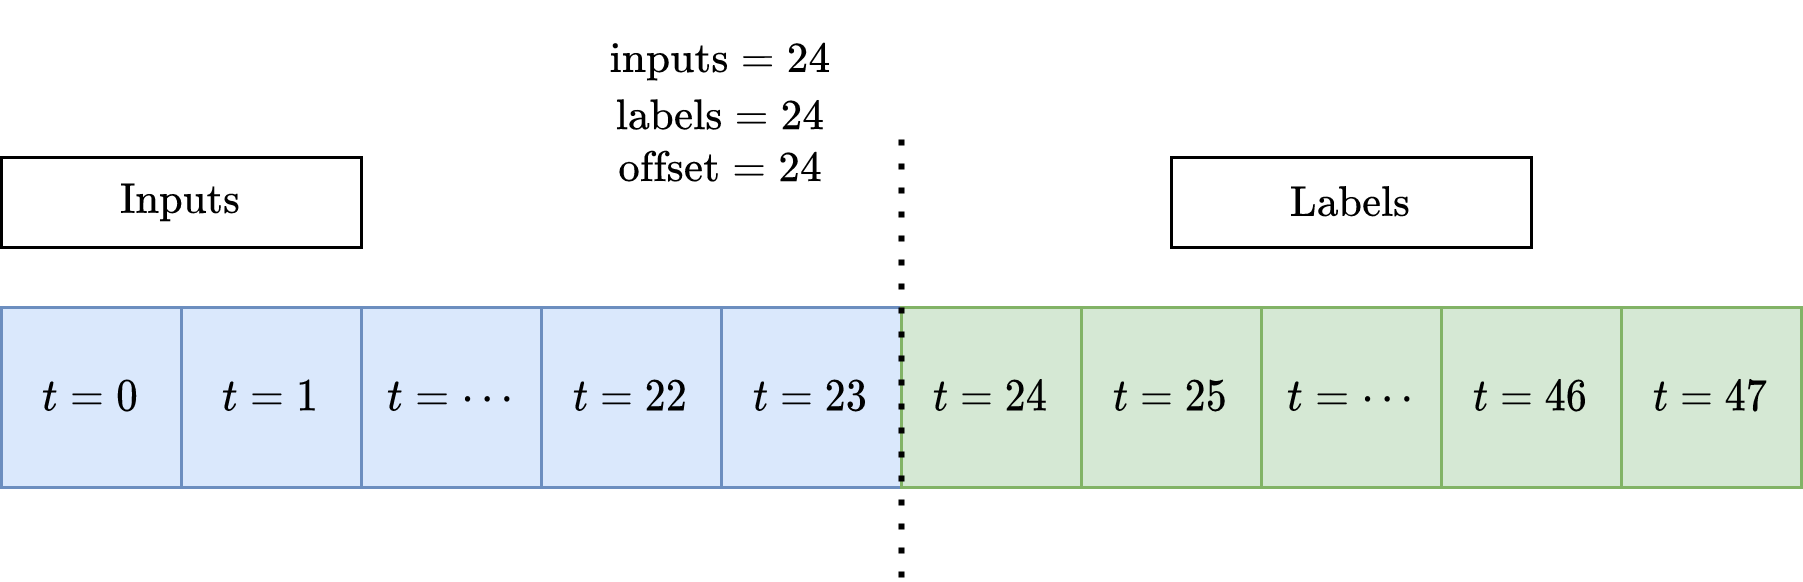
\includegraphics[width=12cm]{images/solution/modules/windows/windows-1.png}
    \caption{Window with a multiple inputs and multiple outputs.}
\end{figure}


\begin{figure}[H]
    \centering
    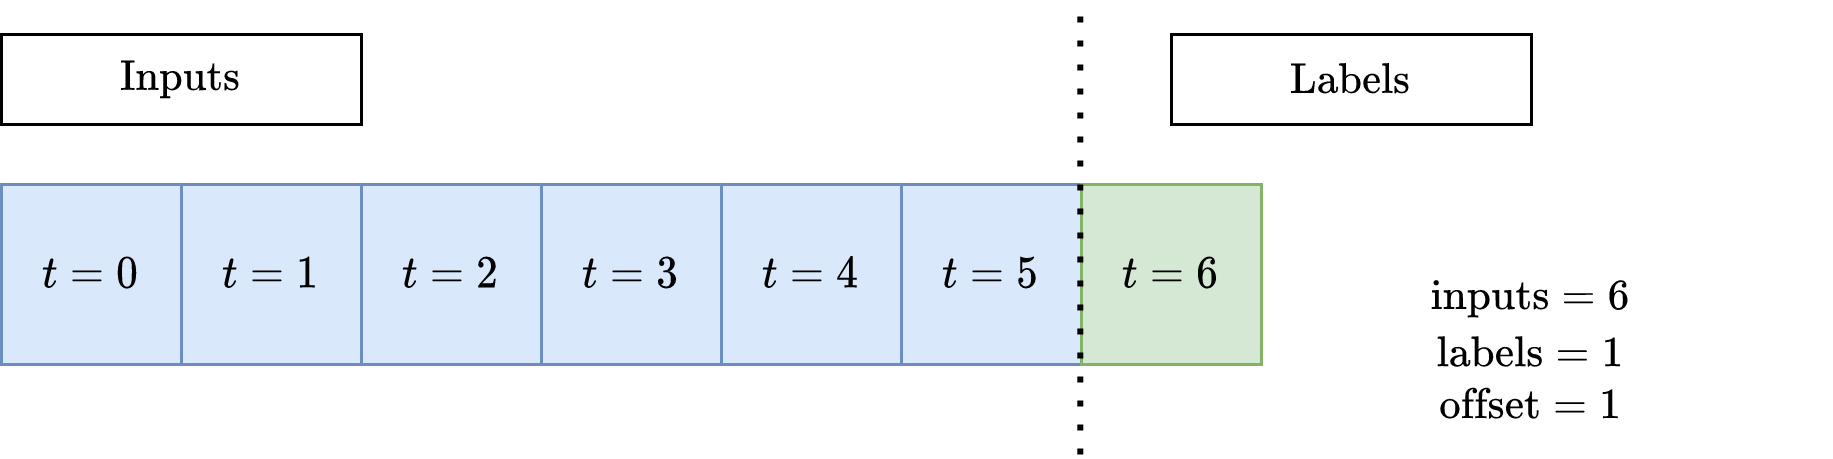
\includegraphics[width=12cm]{images/solution/modules/windows/windows-2.png}
    \caption{Window with a single output interval.}
\end{figure}



\begin{figure}[H]
    \centering
    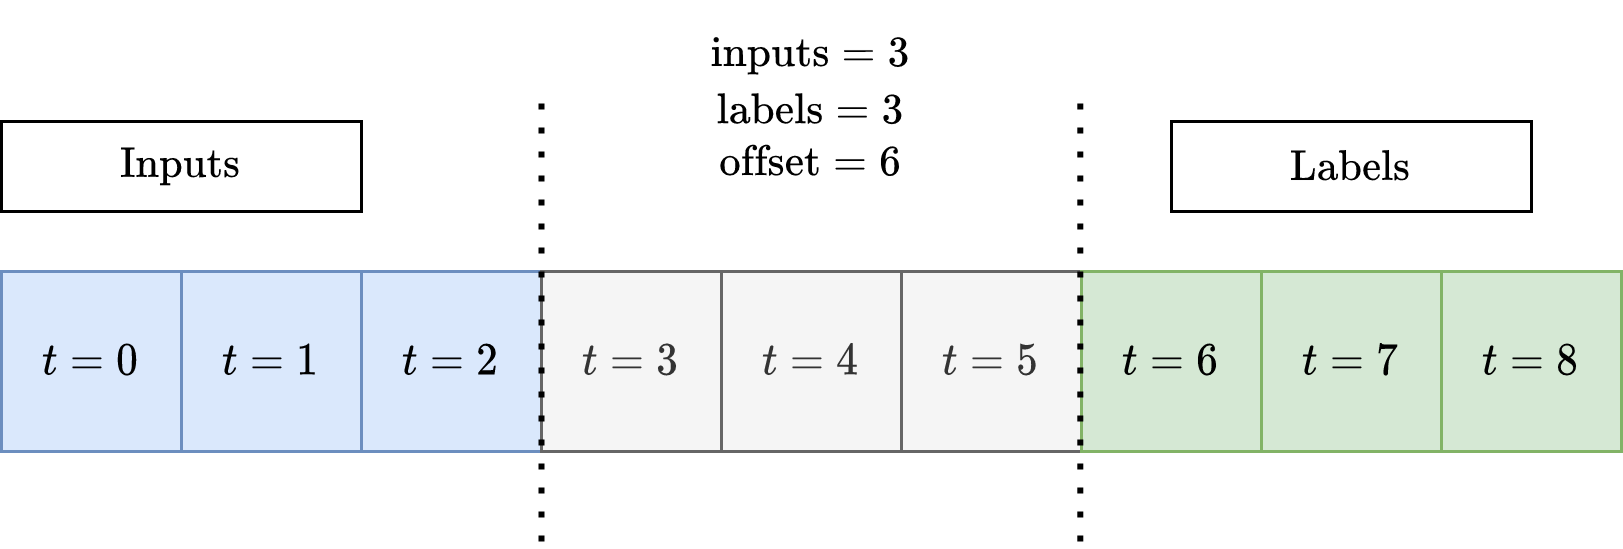
\includegraphics[width=12cm]{images/solution/modules/windows/windows-3.png}
    \caption{Window with offset.}
\end{figure}

Each box represents an interval. The blue colour represents that they will be intervals that the model will use as input, each blue box has an associated vector with \small{\verb|hour|}\normalsize, \small{\verb|day_of_week|}\normalsize, \small{\verb|month|}\normalsize, and the number of trips started for all stations in that interval. All the vectors that represent the input intervals, as explained in section \ref{inputs-outputs}, will be transformed into a single dimensional vector. The green boxes on the other hand represent the intervals that the neural networks will predict. For each interval, a vector will be created with as many elements as stations in the system, being each value the prediction for each station.
\newline


Predictions on the other hand can be made in two different ways:

\begin{itemize}
    \item Single prediction: Given a set of input data, all predictions will be made from these data in a single iteration.
    
    \begin{figure}[H]
    \centering
    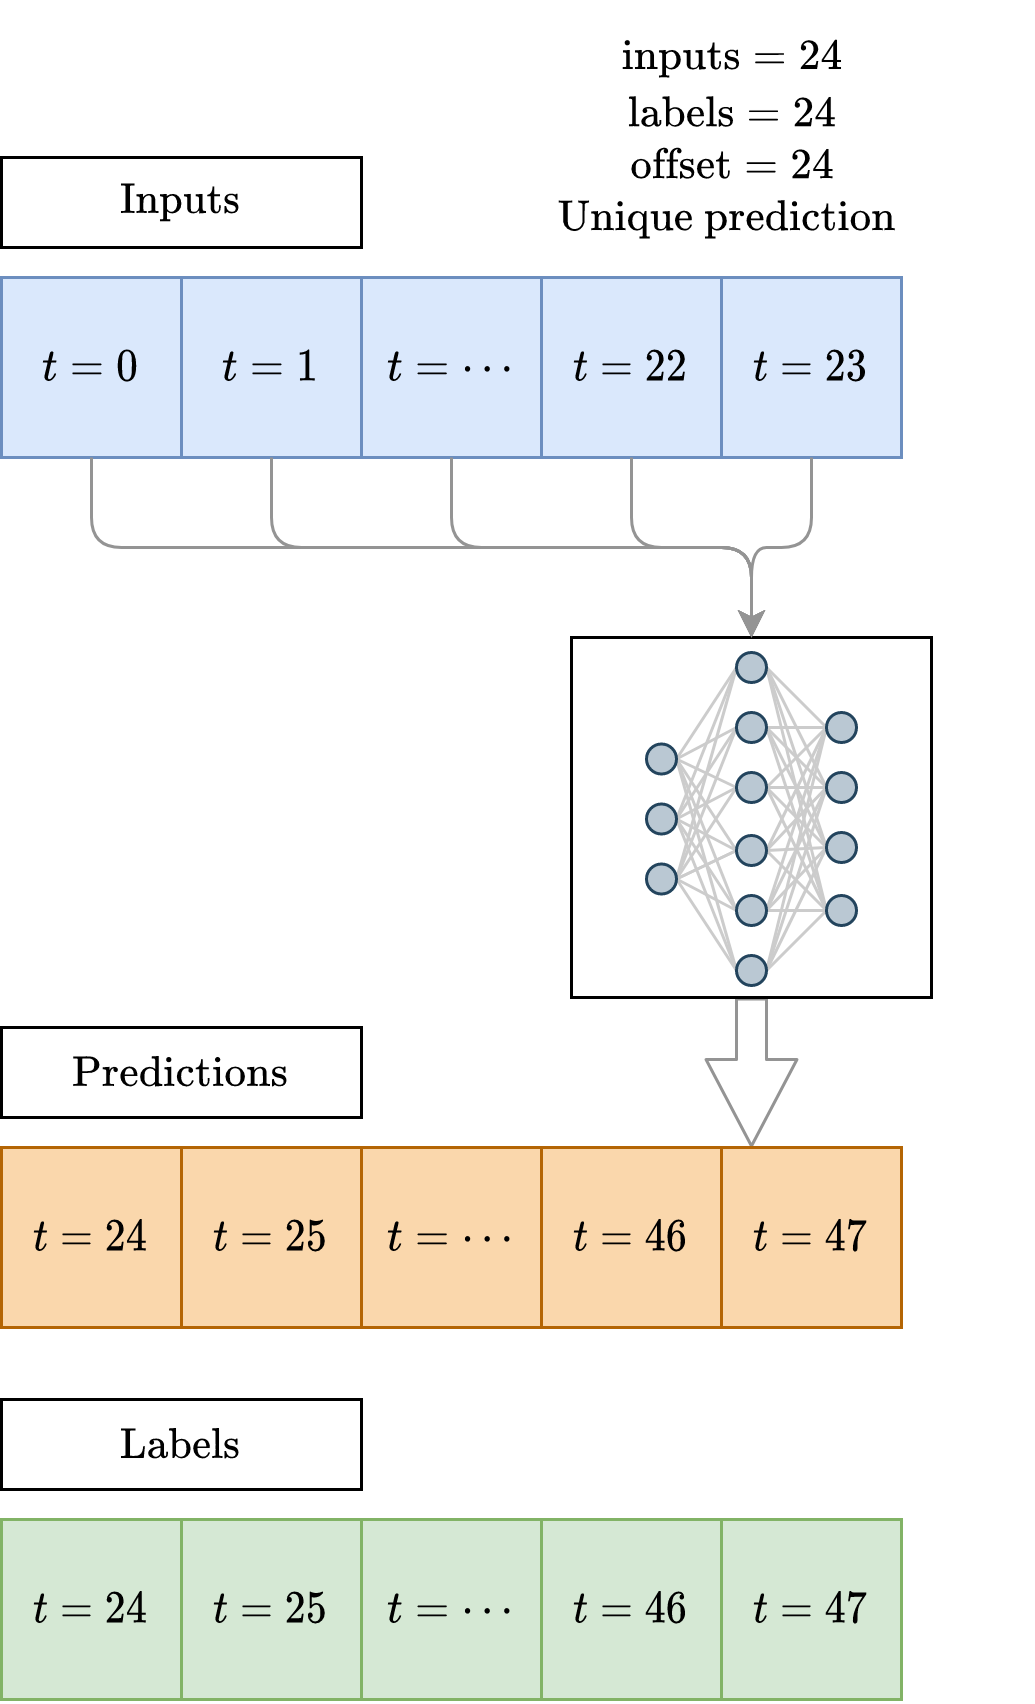
\includegraphics[width=7cm]{images/solution/modules/windows/windows-predictions-one-shot.png}
    \caption{Unique predictions.}
    \end{figure}

    \item Auto-regressive prediction \label{window_ar}: The prediction of the nearest interval in the future will be made first. This prediction will be used together with a state vector in order to calculate the next prediction. Viewed graphically:
    \begin{figure}[H]
    \centering
    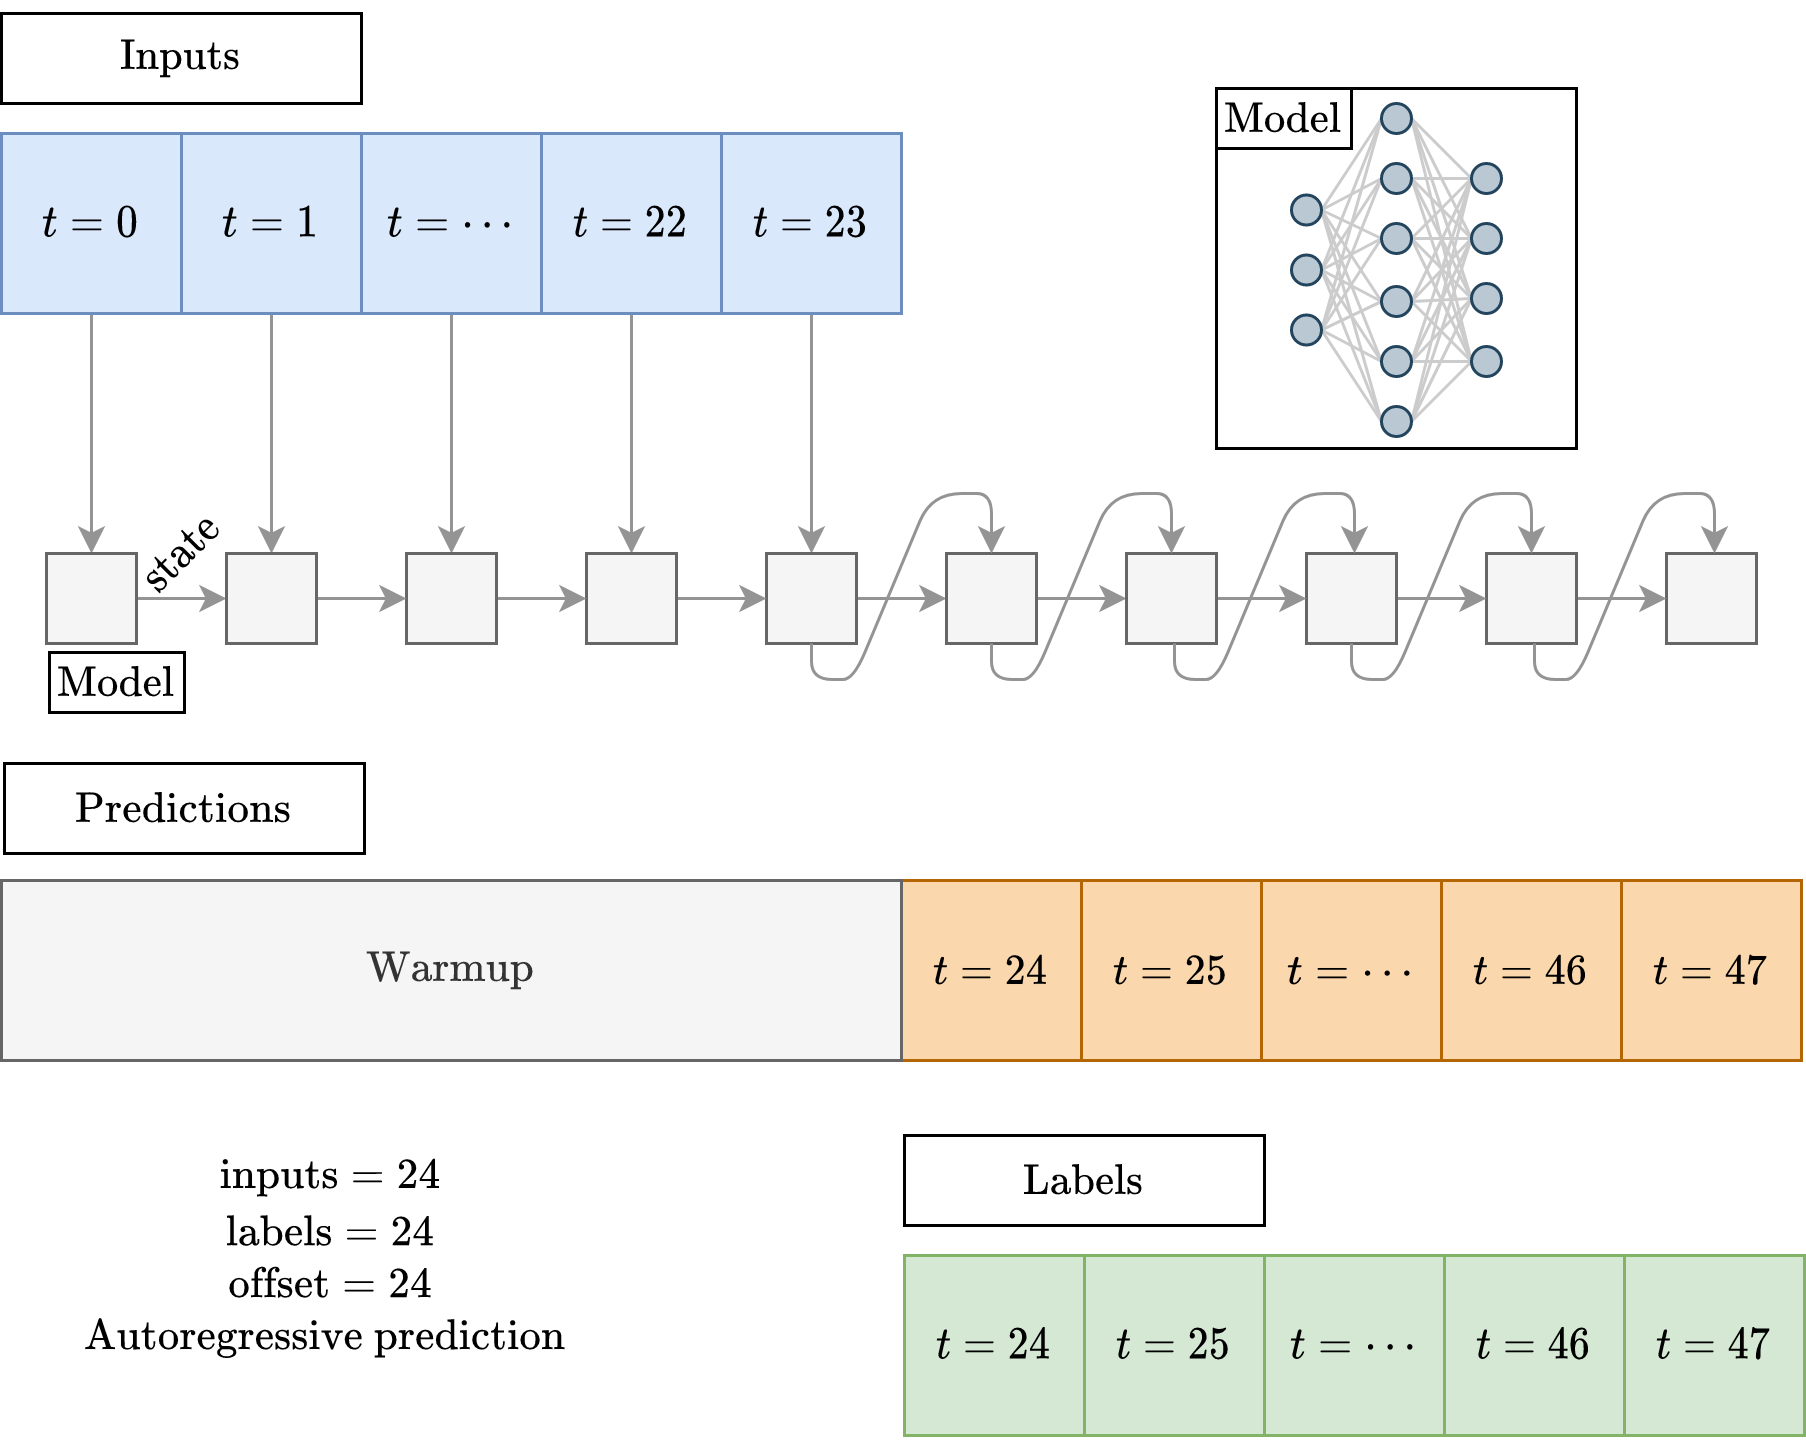
\includegraphics[width=12cm]{images/solution/modules/windows/windows-predictions-ar.png}
    \caption{Autoregressive prediction.}
    \end{figure}
\end{itemize}

Once you have the windows, you must make the window slide and thus generate new vectors that will serve for training. Let us say, for example, that you have a dataset with 7 intervals. You want to train a model that receives 3 input intervals and 1 output interval. Therefore, the model will be trained with a batch of size 4:


\begin{figure}[H]
    \centering
    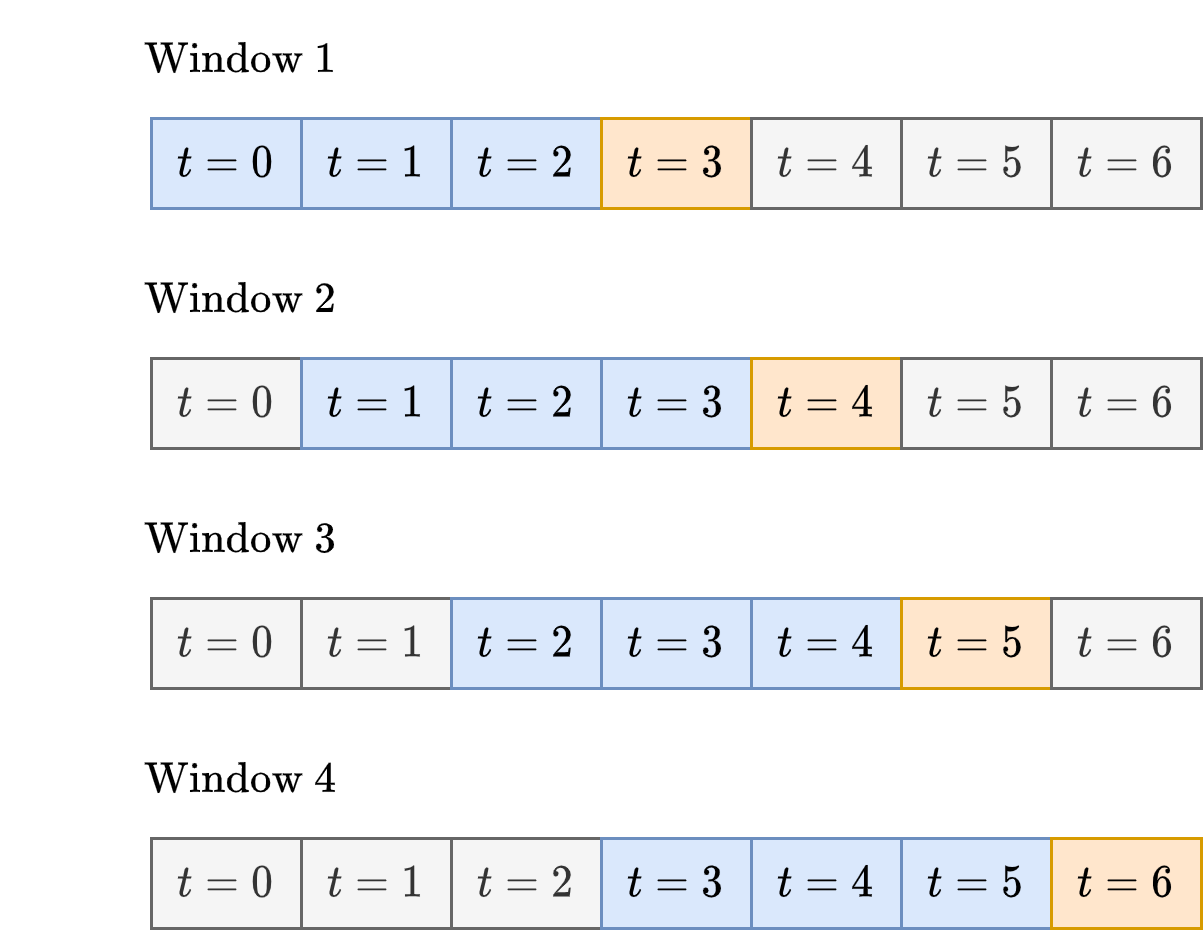
\includegraphics[width=7cm]{images/solution/modules/windows/sliding-windows.png}
    \caption{Behaviour of a sliding window..}
\end{figure}


\subsubsection{Window Generator Code}\label{window-generator-code}


For this module, a class has been generated to create objects and it is based largely on the official Tensorflow tutorial \cite{tensorflow2015-whitepaper} that has been modified to meet the needs of the project. The code used can be seen in Appendix \ref{app:window_generator}.
\newline

All the methods used in the class are explained in detail below:


\begin{itemize}
    \item Indexes and offsets: The \small{\verb|__init__|} \normalsize method (Python constructor) includes all the necessary logic for input and label indexes. It also takes the training, validation and test \small{\verb|DataFrames|} \normalsize as input. These will be converted to \small{\verb|tf.data.Datasets|} \normalsize later. Finally, it receives the index of the column where the temporary information is located. This index is a value equal to $-3$, because as you can see in table \ref{tab:intervals_example}, the last three columns are the ones that contain information about the time, day of the week and month.
    
    \item Splitting the window between input and label: Given a list of consecutive intervals, the \small{\verb|split_window()|} \normalsize method will turn into an input window and a label window.

    
    \item Creation of \small{\verb|tf.data.Datasets|} \normalsize: The \small{\verb|make_dataset()|} \normalsize method will take an interval \small{\verb|DataFrame|} \normalsize and convert it into a pair \small{\verb|tf.data.Dataset|} \normalsize (\small{\verb|input_window|} \normalsize, \small{\verb|label_window|} \normalsize). Size 32 batches have been used.
    
    
    \item The \small{\verb|WindowGenerator|} \normalsize class contains the training, validation and test \small{\verb|DataFrames|}\normalsize. At the end, the properties to access them are added, which are of type \newline\small{\verb|tf.data.Datasets|} \normalsize that make use of the previous method \small\verb|make_dataset|\normalsize.

\end{itemize}